\documentclass[12px]{article}

\title{Lezione 5 Geometria 2}
\date{2025-03-10}
\author{Federico De Sisti}

\input{../../../setup.tex}

\begin{document}
	\maketitle
	\newpage
	\subsection{Funzioni continue}
	\textbf{Osservazione}\\
	Siano $X,Y$ spazi topologici, $f: X \rightarrow Y$.\\
	Siano $A\subseteq Y$ un sottoinsieme,
	 \[
		 X\setminus f^{-1}(A) = \{x\in X \ | \ f(x)\not\in A\} = \{x\in X | f(x) \in Y\setminus A\} = f^{-1}(Y\setminus A)
	.\] 
	Analogamente, con $A,B\subseteq Y$ e $C,D\subseteq X$
	\[
	 f^{-1}(A\cup B) = f^{-1}(A)\cup f^{-1}(B)
	.\] 
	\[
	f^{-1}(A\cap B) = f^{-1}(A)\cap f^{-1}(B)
	.\] 
	\[
	 f(C\cup D) \neq f(C)\cup f(D)
	.\] 
	\[
	 f^{-1}(f(C))\supsetneq C
	.\] 
	\[
	 f(f^{-1}(A)) = A\cap Im(f)
	.\] 
	Tornando a $f: X \rightarrow Y$\\
	$f$ continua $ \Leftrightarrow f^{-1}(A)$ aperto $\forall A\subseteq Y$ aperto $ \Leftrightarrow X\setminus f^{-1}(A) = f^{-1}(Y\setminus A) $ chiuso \ \ $\froall A\subseteq Y$ aperto $ \Leftrightarrow$ con $C = Y\setminus A$ $f^{-1}(C)$ chiuso $\forall C\subseteq Y$ chiuso.
	\begin{defi}[Continuità]
		Sia $f:X \rightarrow Y$ applicazione fra spazi topologici. Sia $p\in X$,  $f$ è continua in $p$ se
		\[
			\forall U\subseteq Y\text{ intorno di } f(p) \ \exists V\subseteq X \text{ intorno di } p \text{ t.c } f(V)\subseteq U
		.\] 
	\end{defi}

	\begin{teo}
		Sia $f:X \rightarrow Y$ applicazione fra spazi topologici, sono equivalenti:
\begin{enumerate}
	\item $\forall p\in X:\  f$  è continua in $p$
	\item  $\forall Z\subseteq X: \ f(\bar Z)\subseteq \overline {f(X)}$  
	\item $f$ continua
\end{enumerate}
	\end{teo}
	\begin{dimo}
		$1) \Rightarrow 2)$ Sia $p\in \overline Z$ so che  $f$ è continua in $p$.\\
		Voglio dimostrare che 
		 \[
		 f(p)\in \overline{f(Z)}
		.\] 
		Formuliamo questa condizione in termini di intorni:\\
		devo dimostrare che in ogni intorno di $f(p)$ ci sono punti di  $f(Z)$. Sia $U\subseteq Y$ intorno di  $f(p)$ per continuità in $p$ $\exists V\subseteq X$intorno di  $p$ tale che $f(V)\subseteq V$ \\
		Visto che $p\in \overline Z$ esiste  $z\in Z$ tale che $z\in V$\\
		Allora  $f(z)$ è in $U$ e in $f(Z)$\\
		cioè ogni intorno $U$ di $f(p)$ contenente punti di $f(Z),$ cioè $f(p)\in \overline{f(Z)}$\\[10px]
		$2) \Rightarrow 3)$ Dimostriamo che $f^{-1}(C)$\\
		è chiuso  $\forall C\subseteq Y$ chiuso. Considero $f^{-1} (C)$, voglio dimostrare che è chiuso confrontandolo con  $\overline{f^{-1}(C)}$.\\
		L'ipotesi 2) dice:
		 \[
			 f(\overline{f^{-1}(C)})\subseteq\overline{f(f^{-1}(C))} = \overline{C\cap f(X)}\subseteq C
		.\] 
		Dato che $C$ è un chiuso che contiene $C\cap f(X)$\\
		Allora  $\overline{f^{-1}(C)}\subseteq f^{-1}(C)$\\
		D'altronde vale sempre  $\overline{f^{-1}(C)} \supseteq f^{-1}(C)$\\
		quindi  $\overline{f^{-1}(C)}= f^{-1}(C)$\\
		da cui  $f^{-1}(C)$ è chiuso.\\[10px]
		$3) \Rightarrow 1)$ suppongo $f$ continua, sia $p\in X$, sia $U\subseteq Y$ intorno di $f(p)$ scegliamo $a\subseteq Y$ aperto con $f(p)\in A \subseteq U$\\
		per continuità:
		$f^{-1}(A)$ aperto di $X$ e contiene  $p$,\\
		posso prendere  $V = f^{-1}(A)$, intorno aperto di $p$, ed è tale che  $f(V)\subseteq A\subseteq U$\\
	\end{dimo}
	\begin{prop}
		La composizione di applicazioni continue qualsiasi è continua
	\end{prop}
	\begin{dimo}
		Siano $X \xrightarrow{f}{} Y \xrightarrow{g}{}Z$\\
		applicazioni fra spazi topologici, suppongo $f\circ g$ continue,\\
		dimostriamo che $g\circ f$ è continua.\\
		Sia $Z$ aperto dimostriamo che
		\[
		 (g\circ f)^{-1}(A) \text{ è aperto } 
		.\] 
		\[
			(g\circ f)^{-1}(A) = \{x\in X \ | \ (g\circ f)(x)\in A\}
		\] 
		\[
			= \{x\in X \ | \ f(x) \in g^{-1}(A)\} = f^{-1}(g^{-1}(A))
		.\] 
		$g$ manda aperti in aperti, stesso per $f$, segue che la composizione fa lo stesso.
	\end{dimo}
	\newpage
	\begin{defi}
		Siano $X,Y$ spazi topologici, $f : X \rightarrow Y$.
		\begin{enumerate}
			\item $f$ si dice omeomorfismo se $f$ è continua, biettiva, e $f^{-1}:Y \rightarrow X$ è continua
			\item $X$ e $Y$ si dicono omeomorfi se esiste $f: X  \rightarrow Y$ omeomorfismo
			\item $f$ (non necessariamente omeomorfismo, non necessariamente continua) si dice aperta se $f(A)$ è aperto $\forall A\subseteq X$ aperto, e  $f$ si dice chiusa quando $f(C)$ è chiuso $\forall C\subseteq X$ chiuso
		\end{enumerate}
	\end{defi}
	\textbf{Esempi:}\\
	$\R$ con topologia euclidea, $f : \R \rightarrow\R$ applicazione costante $f(x) = q \ \ \forall x\in \R$.\\
	Questa $f$ non è aperta, perché $\R$ è aperto in $\R$ e  $f(\R) = \{q\}$ non è aperto in topologia euclidea.\\
	\textbf{Esempio importante:}\\
	Applicazione non chiusa.\\
	\begin{aligned}
		$p : &\R^2 \rightarrow\R$\\
		$(x&,y) \rightarrow x$
	\end{aligned}\\
	$(\R^2, \R$ con topologia euclidea $)$\\
	Non è chiusa, prendiamo ad esempio  $C = \{(x,y) \ | \ x\cdot y = 1\}$\\
	è un chiuso in $\R^2$, ma $p(C) =   \R\setminus\{0\}$ non è chiuso.\\

	$C$ è chiuso di  $\R^2$ perché $C$ è uguale a $f^{-1}(\{1\})$ dove \\
	\begin{aligned}
		$f:\R^2 &\rightarrow\R$\\
		$(x,y)	& \rightarrow xy$
	\end{aligned}\\
	Infatti $f $ è continua e $\{1\}\subseteq \R$ è un chiuso.\\
	\subsection{Spazi metrici}
	\begin{defi}
		sia $X$ un insieme e $d:X\times X \rightarrow\R$\\
		$d$ si dice distanza se:
		\begin{enumerate}
			\item $d(x,y)\geq 0 \ \ \forall x,y\in X,$\\ 
				$d(x,y) = 0 \Leftrightarrow x = y$
			\item $d(x,y) = d(y,x) \ \ \forall x,y\in X$
			\item $d(x,z)\leq d(x,y) + d(y,z)$\\
				 $\forall x,y,z\in X$
		\end{enumerate}
		In tal caso $(X,d) (o X$ stesso $)$ si chiama spazio metrico
	\end{defi}
	\textbf{Esempio}\\
	Sia $X$ insieme, poniamo
	\[
	 d(x,y) = \begin{cases}
		 0 \ \ \text{ se } x = y\\
		 1 \ \ \text{ se } x \neq y
	 \end{cases}
	.\]
	$d$ è una distanza.
	\begin{defi}
		Sia $(X, d)$ spazio metrico.
		\begin{enumerate}
			\item La \underline{palla aperta} di centro $x$ e raggio $\varepsilon\in \R_{>0}$ è: \\$B_\varepsilon(x) = \{p\in X \ | \ d(p,x) < \varepsilon\}$ 
			\item La \underline{topologia indotta} da $d$ su $X$ è definita da:\\
				 $A$ aperto $ \Leftrightarrow \ \forall a\in A\ \exists \varepsilon < 0 \ | \ B_\varepsilon (a)\subseteq A$\\
				 La denotiamo con $T_d$
		\end{enumerate}
	\end{defi}
	Verifica che $T_d$ è topologia
	\begin{enumerate}
		\item $\emptyset, X$ sono aperti: ovvio
		\item unione di aperti è aperto: ovvio
		\item Siano $A_1, A_2\in T_d$, verifichiamo che $A_1\cap A_2\in T_d$, sia $a\in A_1\cap A_2$ quindi $\exists \varepsilon > 0 \ | \ B_\varepsilon (a)\subseteq A_1$ e $\exists \delta > 0 \ | \ B_\delta(a)\subseteq A_2$\\
			sia $\gamma = \min\{\varepsilon, \delta\}$ allora soddisfa  $B_\gamma (a)\subseteq A_1\cap A_2$
	\end{enumerate}
	\begin{lemm}
		Sia $(X,d)$ spazio metrico e $T_d$ la topologia indotta da $d$ 
		\begin{enumerate}
			\item $\forall p\in X \ \forall \varepsilon > 0 \ \ B_\varepsilon (p)\in T_d $
			\item $B = \{B_\varepsilon (p) \ | \ p\in X, \varepsilon \in \R_{>0}\}$\\
				è una base di  $T_d$ 
			\item Un sottoinsieme $U\subseteq X$ è intorno di $p\in X$ se e solo se \\ $\exists \varepsilon > 0 \ | B_\varepsilon(p)\subseteq U$
		\end{enumerate}
	\end{lemm}
	\begin{dimo}
		Per esercizio.
	\end{dimo}
	\textbf{Osservazione}\\
	Gli spazi metrici in generale si comportano in modo simile a $\R& n$ con distanza euclidea, ma attenzione: non tutto è uguale, ad esempio se $(X,d)$ è uno spazio metrico e $x\in X:$
	 \[
		 \{p\in X \ | \ d(x,p)\leq \varepsilon\}
	.\] 
	con $\varepsilon > 0 $ fissato, è un chiuso di $X$ (verifica per esercizio) ma non è sempre la chiusura di $B_\varepsilon (x)$.\\
	Ad esempio  $X = \R$ con distanza  $d(x,y) = \begin{cases}
		0\ \  \text{ se } x = y\\
		1 \ \ \text{ se } x\neq y
	\end{cases}$ \\
	Considero $\{p\in\R \ | \ d(p,x)\leq 1\} = \R$\\
	ma $B_1(x) = \{x\}$\\
	Questo vale  $\forall x\in \R$\\
	cioè ogni ogni singoletto è aperto, allora  $T_d$ è discreta, quindi $\{x\}$ è anche chiuso. Cioè $B_1(x) = \{x\}$.\\
	 \textbf{Osservazione:}\\
	 Siano $X,Y$ spazi metrici sia $p\in X$\\
	  $f: X \rightarrow Y$, allora $f$ è continua in $p$\\
	   $($ come applicazione fra spazi topologici, dove su $X $ e $Y$ metto le topologie indotte dalle distanze) $ \Leftrightarrow \  \forall \varepsilon > 0 \ \ \exitsts \delta > 0 \ | \ $ se $d(x,p) < \delta$ allora  $d(f(x),f(p)) < \varepsilon$\\
	   Verifica per esercizio
	   \begin{coro}
	   	Siano $d, h$ distanze su uno stesso insieme $X.$\\
		Allora  $T_d$ è più fine di $T_h$ se $\forall p\in X \ \ \forall \varepslion > 0\ \ \exists \delta > 0 \ |  \ B_\delta^d(p)\subseteq B_\varepsilon ^h(p)$
	   \end{coro}
	   \begin{dimo}
	   	Usiamo $id_X: X \rightarrow X$ dove nel dominio prendiamo $d$ e $T_d$, e nel codominio la distanza $h$ e $T_h$. Con questa scelta l'identità su $X$ è continua $ \Leftrightarrow$ $T_d\supseteq T_h$\\
		La carindalità di  $Id_X$ è equivalente alla condizione con $\varepsilon$ e $\delta$ per l'osservazione.
	   \end{dimo}
	   \begin{defi}[Distanze equivalenti]
	   	Date distanze $d,h$ su un insieme $X$, esse si dicono equivalenti se $T_d = T_h$
	   \end{defi}
	   \begin{defi}[Spazio topologico metrizzabile]
	   	Sia $X$ uno spazio topologico con topologia $T$. Se esiste una distanza $d$ su $X$ tale che $T = T_d$ allora $X$ si dice metrizzabile.
	   \end{defi}
	   \subsection{Sottospazi topologici}
	   \begin{defi}
	   	Sia $X$ spazio topologico, sia $Y\subseteq X$ sottoinsieme qualsiasi, allora su $Y$ è definita la topologia di sottospazio ponendo $A\subseteq Y$ aperto in topologia di sottospazio $ \Leftrightarrow$ $\exists B\subseteq X$ aperto in $X$ tale che $A = B\cap Y$
	   \end{defi}
	   \textbf{Esempi:}\\
	   1) $X = \R$ con topologia euclidea\\
	   $Y = [0,1]$\\
	   Allora  $Y$ è aperto in topologia di sottospazio\\
	   $A = Y$ soddisfa $A = B\cap Y$\\
	   Anche  $I = ]\frac 12 , \frac 23[\subseteq Y$ è aperto in topologia di sottospazio basta prendere  $B' = I$ per avere  $I = B'\cap Y$ \\
	   Considero $[0,\frac 12[ = J\subseteq Y$\\
	   non è aperto in  $\R = X$, ma è aperto in  $Y$ in topologia di sottospazio, basta prendere $B''=]-1,\frac 12 [ $ è aperto in  $X$ e soddisfa
	   \[
	    J = B''\cap Y
	   .\] 
	   Idea intuitiva:
	   %TODO fixa immagine 10 marzo 5 39
	  \begin{center}
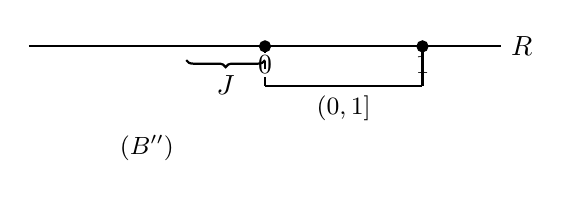
\begin{tikzpicture}

    % Draw the real line
    \draw[thick] (-3,0) -- (3,0);
    
    % Interval J
    \draw[thick, decoration={brace, mirror, raise=5pt}, decorate] (-1,0) -- (0,0) node[midway, below=7pt] {$J$};
    
    % Points on the line
    \filldraw (0,0) circle (2pt) node[below] {$0$};
    \filldraw (2,0) circle (2pt) node[below] {$1$};

    % Bracket for the interval (0,1]
    \draw[thick] (0,-0.5) -- (2,-0.5);
    \draw[thick] (2,-0.5) -- (2,0);
    \draw[dashed] (0,-0.5) -- (0,0);

    % Labeling the interval
    \node[below] at (1,-0.5) {\small $(0,1]$};
    \node[right] at (3,0) {$\mathbb{R}$};

    % Additional notation B''
    \node[below] at (-1.5,-1) {\small $( B'' )$};

\end{tikzpicture}
\end{center}

	   $J$ non è aperto in $\R$ perché  $\forall\varepsilon > 0 \exists$ punti di $\R$, a distanza $< \varepsilon$ da $0$, punti che non sono in $J$.\\
	   Ma  $J$ aperto in $Y$ in topologia di sottospazio perché $Y$ non contiene tali punti\\
	   2) $X = \R$ con topologia euclidea, sia $Y = \Z$ con topologia di sottospazio, Ad esempio  $A = ]-100, 23[\cap Y = \{-99,-98,\ldots,22\}$\\
	   Anche $]-\frac 12, \frac 12[\cap \Z = \{0\}$ è aperto.\\
	   Analogamente\\
	   $]n - \frac {12}, n + \frac 12[\cap \Z = \{n\} \ \ \forall n\in \Z$ è aperto in  $\Z$ in topologia di sottospazio. Quindi la tipologia di sottospazio è discreta.\\
	   3) $X = \R^2$ con topologia euclidea, $Y = \R \times \{0\}$, l'asse  $x.$\\

\begin{center}
\begin{tikzpicture}[scale=1]
    % Draw the x-axis
    \draw[->] (-1,0) -- (2,0) node[right] {$x$};

    % Draw the y-axis
    \draw[->] (0,-1) -- (0,2) node[above] {$y$};

    % Highlight a segment on the x-axis (e.g., [0,1])
    \draw[very thick] (0,0) -- (1,0);

    % Label points
    \fill (0,0) circle (2pt) node[below left] {$0$};
   \fill (1,0) circle (2pt) node[below] {$1$};

    % Indicate open boundary at 1
    \draw (1,0) circle (2pt);
\end{tikzpicture}
\end{center}
	   allora  $A = ]0,1[\times\{0\}$ è aperto in topologia di sottospazio, ad esempio  $B = ]0,1[\times\R$\\
	   %TODO aggiungi immagine 10 marzo 5 47\\
	   \textbf{Osservazione} Verifichiamo che la topologia di sottospazio è una topologia:
	   \[
		   T_Y = \{A\subseteq Y \ | \ \exists B\subseteq X \ \text{ aperto t.c.}  B\cap Y = A\}
	   .\] 
	   Assiomi di topologia
	   \begin{enumerate}
		   \item $\emptyset = \emptyset \cap Y$,  $Y = X\cap Y$
		   \item Siano  $A_i, i\in I$ elemento di  $T_Y$, verifica che  $ \bigcup^{}_{i\in I}A_i$ è in $T_y$\\
			   Scegliamo  $B_i \ \ \forall i\in I$ aperto in  $X$ t.c. \ $ A_i = B_i\cap Y$\\
			    $ \bigcup^{}_{i\in I}A_i = \bigcup^{}_{i\in I}(B_i\cap U) = \bigcup^{}_{i\in I}B_i\cap Y$ dove il primo termine è aperto in X\\
			    da cui $  \bigcup^{}_{i\in I}A_i \in T_Y$.\\
		    \item Siano $A_1, A_2\in T_Y$, scegliamo $B_1,B_2$ aperti in $X$ con $A_i = B_i\cap Y \ \ \forall i\in \{1,2\}$ allora \\
			     $A_1\cap A_2 = (B_1\cap Y)\cap (B_2\cap Y) = B_1\cap B_2)\cap Y$ dove il primo termine è aperto in $X$\\
			     quindi $A_1\cap A_2\in I_y$\\
	   \end{enumerate}
			    \textbf{Osservazione.}\\
		 Sia $C\subseteq Y$ chiuso in topologia di sottospazio. Allora $A = Y\setminus C$ è scrivibile come $A = B\cap Y$ con $B$ aperto in $X$, Allora $D = X\setminus B$ è chiuso in $X, $ e vale $D \cap Y = C$\\
		 Cioè se  $C $ è chiuso in topologia di sottospazio allora esiste $D\subseteq X$ chiuso tale che  $C = D\cap Y$.\\
		 Vale il viceversa se il sottoinsieme  $C$ di $Y$ è scrivibile come  $C = D\cap Y$ con $D \subseteq X$ chiuso, allora  $C$ è chiuso in topologia di sottospazio (esercizio)

\end{document}
